For the system below, define two reference frames for the system using orthogonal unit vectors

\begin{center}
    
\includegraphics[width=0.75\textwidth]{img/fig24_7.png}
\end{center}

\begin{enumerate}
    \item One reference frame will be known as the “global frame” and defined by the unit vectors $\left[\hat{i}, \hat{j}\right]$. The $\hat{i}$ vector should be parallel to the floor, with the $\hat{j}$ vector perpendicular to the floor.
    \item The second reference frame will be known as the “ramp frame” and defined by the unit vectors $\left[\hat{x}, \hat{y}\right]$. The $\hat{x}$ vector should be parallel to the ramp, with the $\hat{y}$ vector perpendicular to the ramp.
\end{enumerate}

\begin{solution}\
\begin{center}
    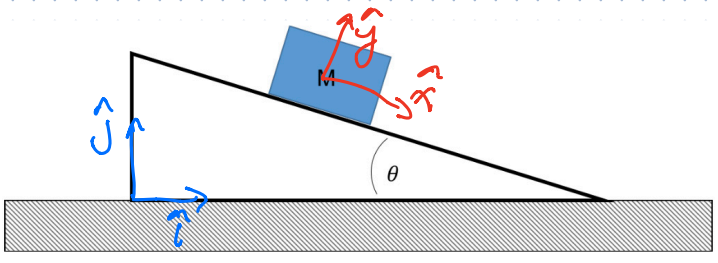
\includegraphics[width=0.75\textwidth]{img/e9p1.png}
\end{center}
\end{solution}
